\documentclass[11pt]{article}
\usepackage{amsmath,textcomp,amssymb,geometry,graphicx,enumerate,float}
\graphicspath{{../../lab_analog/plots/}}

\def\Name{Jeff Lievense}  % Your name
\def\HW{1} % Homework number

\title{Astronomy 121 -- Spring 2014}
\author{\Name}
\markboth{Astronomy 121 -- Spring 2014, Lab \HW, \Name}{Astronomy 121 -- Spring 2014, Lab \HW, \Name}
\pagestyle{myheadings}

\begin{document}
\maketitle
\begin{center}
{\LARGE
{\bf Lab 1 \\~\\

Impedance, Filters, Amplifiers, and Noise
}
}
\end{center}

\newpage
\section{Abstract}
In this report, we develop the necessary theory and tools for designing and implementing radio receiver circuits. RLC filters are developed from the concepts of impedance and voltage division. FM-to-AM conversion via band-pass filtering is described, and strategies for AM demodulation are given. Basic transistor amplifier are described as well as their purpose in an FM demodulator. We also discuss the effects of transmission lines and noise.

\section{Introduction}
In order to use electronics to make measurements about radio frequency (RF) signals, we must understand how these things interact with each other. This involves understanding how we can use electronics to acquire RF signals, what kind of RF signals exist and how we can use electronics to decipher them, and what sort of non-ideal and undesirable things electronics can introduce to RF signals. In this lab, we hope to scratch the surface of these topics in order to develop a general sense of comfort when working with RF electronics.

\section{Theory}
In this section, we discuss the theory used in the development of our circuit.

    \subsection{Frequency Modulation}
    We are interested in building a circuit which can recover message signals that have been transmitted via \emph{frequency modulation} (FM). Modulation refers to the message signal being encoded in a very high-frequency \emph{carrier signal} which can travel through free space much farther than the message signal would be able to travel by itself. Frequency modulation means the message is encoded in the frequency of the carrier signal (as opposed to \emph{amplitude modulation} (AM), in which the message signal is multiplied by the carrier signal). Mathematically, we can model an FM signal as
    \begin{flalign*}
        y(t) &= \cos(\omega_c t  + \omega_{\Delta} \int_{0}^t m(t) dt),
    \end{flalign*}
    where $\omega_c$ is the frequency of the carrier signal, $\omega_{\Delta}$ is the frequency deviation, and $m(t)$ is the message signal to be transmitted. $\omega_{\Delta}$ is a design parameter that essentially maps changes in amplitude of the message signal into changes in frequency of the modulated carrier signal. From this definition, we see that an FM signal can be converted to an AM signal via differentiation, that is
    \begin{flalign*}
        \frac{d}{dt}y(t) &= -(\omega_c + \omega_{\Delta}m(t))\sin(\omega_c t + \omega_{\Delta} \int_0^t m(t)dt).
    \end{flalign*}
    From here, the message signal $m(t)$ can be recovered via AM demodulation, which will be discussed in a later section. With this in mind, we will now develop the necessary circuit theory to implement an FM demodulator.

    \subsection{Filters}
    Filtering is the process of eliminating certain frequencies from a signal. When dealing with audio signals such as those transmitted via FM, we often use filters to remove inaudible frequencies, i.e. those that carry no information which can be heard by humans. We will also use filters to approximate differentiation in demodulation, which will be discussed in a later section.

        \subsubsection{Voltage Division}

        \begin{figure}[H]
            \centering
                \includegraphics[width = 200px]{volt_divider.png}
            \caption{A resistive voltage divider.}
            \label{rvd}
        \end{figure}

        \noindent Since a filter is used to eliminate certain frequencies, it must of course contain some components whose functionality is frequency-dependent. However, we must first understand the manner in which electronic components interact with each other. Consider the resistive \emph{voltage divider} in Figure~\ref{rvd}. If some voltage $v_{in}$ is applied at the leftmost terminal, what would the resulting voltage $v_{out}$ at the rightmost terminal be as a function of the resistances in the circuit? We can use Ohm's Law to determine the current $I$ flowing through both resistors and again to determine the voltage drop across $R_2$, which is $v_{out}$. Thus we have
        \begin{flalign*}
            v_{in} &= I\cdot (R_1 + R_2) \\
            I &= \frac{v_{in}}{R_1 + R_2}
        \end{flalign*}
        and
        \begin{flalign*}
            v_{out} &= I\cdot R_2 \\
            &= v_{in} \cdot \frac{R_2}{R_1 + R_2}.
        \end{flalign*}
        We will denote the quantity $\frac{R_2}{R_1 + R_2}$ as the \emph{voltage divider ratio}, as it will appear in many forms in our development of filters.

        \subsubsection{Impedance}
        To build frequency-dependent circuits, we must use components whose impedance is not purely real. We denote the \emph{impedance} of a component as $Z = R + jX$, where $\mathfrak{Re}(Z) = R$ is \emph{resistance} and $\mathfrak{Im}(Z) = X$ is \emph{reactance}. As seen above, the impedance of an ideal resistor is purely real, thus we can characterize a resistor by its resistance. Components such as ideal capacitors and inductors, however, have purely imaginary impedance. We will now derive these imaginary impedances via the Fourier Transform, which will allow us to see the frequency dependence of these components. \\
        \\
        Just as Ohm's Law describes the relationship between current and voltage across a resistor, there are similar expressions for capacitors and inductors. For a capacitor with capacitance $C$ and an inductor with inductance $L$, we have
        \begin{flalign*}
            I &= C\frac{dV}{dt} \\
            V &= L\frac{dI}{dt}.
        \end{flalign*}
        Let $Z = \frac{\mathcal{F}\{V\}}{\mathcal{F}\{I\}}$ be the impedance of some component in the frequency domain, where $\mathcal{F}\{\cdot\}$ denotes the Fourier Transform. Recall that $\mathcal{F}\{\frac{d}{dt}x(t)\} = j\omega X(\omega)$, then we have
        \begin{flalign*}
            \mathcal{F}\{I\} &= C \mathcal{F}\{\frac{dV}{dt}\} \\
            &= C\cdot j\omega \mathcal{F}\{V\} \\
            Z_C &= \frac{1}{j\omega C} \\
            \mathcal{F}\{V\} &= L\mathcal{F}\{\frac{dI}{dt}\} \\
            &= L\cdot j\omega \mathcal{F}\{I\} \\
            Z_L &= j\omega L.
        \end{flalign*}

        \begin{figure}[H]
            \centering
                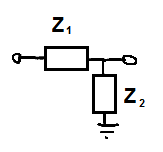
\includegraphics[width = 200px]{imp_divider.png}
            \caption{An arbitrary impedance voltage divider.}
            \label{ivd}
        \end{figure}

        \noindent With this in mind, we can now revisit the voltage divider, but using reactive components instead of resistors. Consider the voltage divider in Figure~\ref{ivd}, where the components are arbitrary impedances. We denote the \emph{transfer function}, or \emph{frequency-dependent gain} of such a circuit to be $H(\omega) = \frac{\mathcal{F}\{v_{in}\}}{\mathcal{F}\{v_{out}\}}$. Returning to the voltage divider ratio from before and replacing resistances with impedances, we have $H(\omega) = \frac{Z_2}{Z_1 + Z_2}$.

        \subsubsection{RC Filters}
        
        \begin{figure}[H]
            \centering
                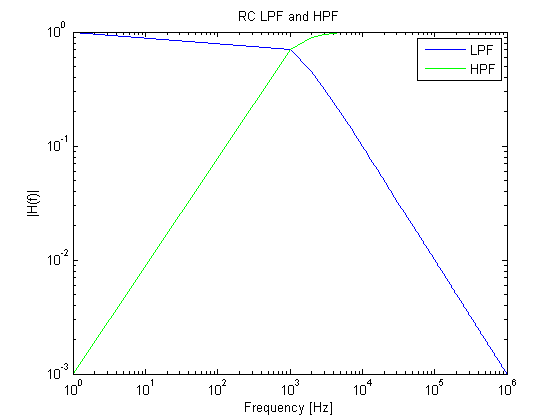
\includegraphics[width = 300px]{rc_matlab.png}
            \caption{Transfer functions for RC LPF and HPF.}
            \label{rcf}
        \end{figure}
        
        Consider the case where $Z_1$ is a capacitor and $Z_2$ is a resistor. The transfer function for such a filter is
        \begin{flalign*}
            H(\omega) &= \frac{R}{\frac{1}{j\omega C} + R} \\
            &= \frac{j\omega R C}{1 + j\omega R C}.
        \end{flalign*}
        We see that $\omega \to 0 \Rightarrow H(\omega) \to 0$ and $\omega \to \infty \Rightarrow H(\omega) \to 1$, therefore we denote this circuit as a \emph{high-pass filter} (HPF), that is, a filter that attenuates signals with low frequencies and passes those with high frequencies (See Figure~\ref{rcf}). To construct a \emph{low-pass filter} (LPF), that is, one which passes signals with high frequencies and attenuates those with low frequencies, we simply switch the order of the resistor and capacitor. Letting $Z_1 = R$ and $Z_2 = \frac{1}{j\omega C}$, we have
        \begin{flalign*}
            H(\omega) &= \frac{1}{j\omega C(R + \frac{1}{j\omega C})} \\
            &= \frac{1}{1 + j\omega R C}.
        \end{flalign*}
        We see that $\omega \to 0 \Rightarrow H(\omega) \to 1$ and $\omega \to \infty \Rightarrow H(\omega) \to 0$, therefore this is indeed a low-pass filter (See Figure~\ref{rcf}). \\
        \\
        An important figure of merit in an RC filter is the \emph{cutoff frequency} $\omega_0$. We define the cutoff frequency to be the frequency at which the power gain $|H(\omega)|^2$ is reduced to half of its passband value $H_0$. That is, $H(\omega_0) = \frac{1}{\sqrt{2}}H_0$. For an RC filter (LPF or HPF), we see that $\omega_0 = \frac{1}{RC}$, where $RC$ is called the \emph{time constant} of the filter.

        \subsubsection{LC Filters}

        \begin{figure}[H]
            \centering
                \includegraphics[width = 200px]{lc_series_parallel.png}
            \caption{Series and parallel combinations of inductors and capacitors.}
            \label{lcsp}
        \end{figure}

        \noindent If we expand our library of components to include inductors, we can achieve different types of filters, such as \emph{band-pass} (BPF) and \emph{band-stop} (BSF) filters. A band-pass filter is a filter that passes all frequencies within a specified band and attenuates everything outside this band, and a band-stop filter does just the opposite. We can construct these filters via series and parallel combinations of capacitors and inductors. \\
        \\
        Consider the parallel combination in Figure~\ref{lcsp}. Its transfer function is given by
        \begin{flalign*}
            H(\omega) &= \frac{1}{j\omega C + \frac{1}{j\omega L}} \\
            &= \frac{j\omega L}{1 - \omega^2 L C}.
        \end{flalign*}

        \begin{figure}[H]
            \centering
                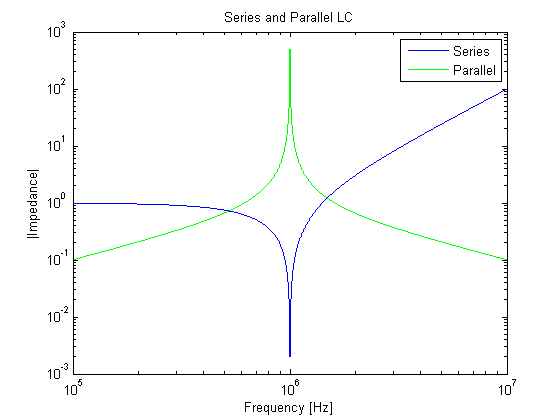
\includegraphics[width = \textwidth]{series_parallel_matlab.png}
            \caption{Impedance versus frequency for series and parallel LC combinations.}
            \label{lcspm}
        \end{figure}

        \noindent From the plot of $H(\omega)$ vs. $\omega$ in Figure~\ref{lcspm}, we see that this is indeed a band-pass filter. Similarly, consider the series combination in Figure~\ref{lcsp}. Its transfer function is given by
        \begin{flalign*}
            H(\omega) &= j\omega L + \frac{1}{j\omega C} \\
            &= 1 - \omega^2 L C.
        \end{flalign*}
        From the plot of $H(\omega)$ vs. $\omega$ in Figure~\ref{lcspm}, we see that this is indeed a band-stop filter. Notice that, in both band-pass and band-stop filters, the filter behaves in an interesting manner when $\omega = \frac{1}{\sqrt{LC}}$. This is no coincidence! Just as we defined the cutoff frequency of an RC filter, we define $\omega_0 = \frac{1}{\sqrt{LC}}$ as the \emph{resonant frequency} of an LC filter. At this frequency, the reactances due to the capacitor and inductor are perfectly out of phase and they "cancel" each other out, yielding interesting results.

        \subsubsection{RLC Filters}
        If we introduce resistance to our LC filters, we can define yet another important quantity. The \emph{quality factor} $Q$ describes the width of the passband or stopband in an RLC filter and is given by $Q = \omega_0 RC = \frac{f_0}{\Delta f_{3dB}}$, where $f_0 = 2\pi\omega_0$ and $\Delta f_{3dB}$ is the width of the passband or stopband. \\
        \\
        Note that RLC filters are \emph{LTI systems}, therefore if we cascade them in series their transfer functions multiply (yielding steeper transitions), and in parallel their transfer functions add.

    \subsection{Diodes}
    We are interested in recovering a nonnegative message signal from a modulated carrier signal. Since carrier signals are zero mean oscillations, we must have some way of ``rectifying'' the carrier signal so the message information can be extracted. We use \emph{diodes} to accomplish this. A diode is a semiconductor component which allows current to flow through it when the voltage drop across it is greater than some threshold, but does not allow current to flow through it otherwise. Since diodes are realized as p-n junctions, they are ``on'' (conducting) when in forward bias and ``off'' (not conducting) when in reverse bias. The aforementioned threshold voltage is thus the built-in potential of the p-n junction, which is usually around 600-700 millivolts.

        \subsubsection{Envelope Detector}

        \begin{figure}[H]
            \centering
                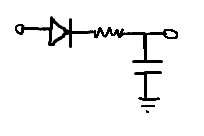
\includegraphics[width = 200px]{env_det.png}
            \caption{An envelope detector.}
            \label{envdet}
        \end{figure}

        \noindent A diode followed by a low-pass filter (see Figure~\ref{envdet}) can be used as an \emph{envelope detector}, if the filter's time constant is chosen correctly. The envelope of a modulated high-frequency carrier signal is the smooth curve which outlines extremes in its amplitude. In the case of AM, the envelope is exactly the desired message signal to be recovered. The diode's rectifying ability turns the modulated carrier signal into a ``choppy'' version of the nonnegative message signal, and the low-pass filter rejects the high-frequency carrier signal, leaving the message signal to be recovered.

    \subsection{Amplifiers}
    In general, a received FM signal will have lost some of its energy in transmission, thus we must be able to amplify it. However, many transistor amplifiers have large output impedances. This is a problem because we are dealing with audio signals, which means there will most likely be a speaker involved. Speakers have very low impedance, so cascading a high output impedance amplifier with a speaker will result in a highly attenuated signal being seen by the speaker. This can be seen from the voltage divider ratio -- if $R_1$ is large and $R_2$ is small, the input signal is attenuated. So, in addition to providing amplification, we must also take into consideration the output impedance of our amplifiers.

        \subsubsection{Gain Stage}
        
        \begin{figure}[H]
            \centering
                \includegraphics[width = 300px]{bjt_amplifier_lab2.png}
            \caption{A common emitter amplifier with resistive biasing and degeneration.}
            \label{ce}
        \end{figure}
        
        \noindent To provide gain, we use the \emph{common emitter} amplifier topology (See Figure~\ref{ce}). With resistive emitter degeneration, this amplifier has DC gain $A_{DC} = \frac{g_m R_C}{1 + g_m R_E}$. Placing a large capacitor in parallel with the degeneration resistor gives a high frequency gain of $A_v = g_m R_C$, because the capacitor shorts out the resistor at high frequencies.

        \subsubsection{Follower}
        
        \begin{figure}[H]
            \centering
                \includegraphics[width = 300px]{biased_emitter_follower.png}
            \caption{An emitter follower amplifier with resistive biasing.}
            \label{cc}
        \end{figure}
        
        To match impedance, we cascade the common emitter with a \emph{common collector}, or \emph{emitter follower} (See Figure~\ref{cc}). An amplifier with this topology has gain $A_v = \frac{g_m R_E}{1 + g_m R_E} \approx 1$, which means it acts as a buffer. Its output impedance is roughly $R_o \approx \frac{1}{g_m} \parallel R_E$, which is designed to be comparable to the low impedance of the load (speaker) in order to avoid loading effects. If we did not follow the common emitter with the emitter follower, the output impedance would be roughly $R_o \approx R_C$, in which case the signal seen by the speaker would be attenuated by a factor of $\frac{1}{R_C}$, hence the name emitter \emph{follower}.

\section{Methods}
In this section we discuss the physical implementation of the theory discussed above.

\begin{figure}[H]
    \centering
        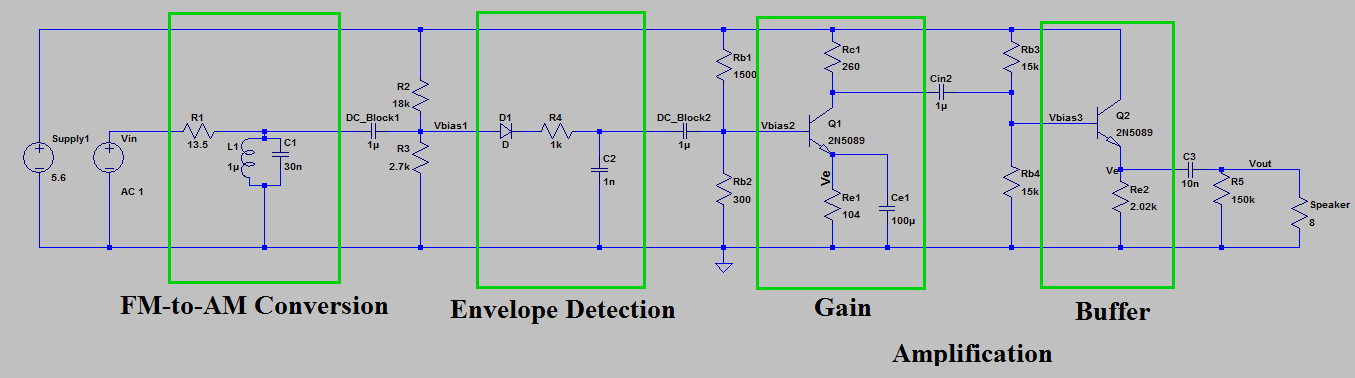
\includegraphics[width = \textwidth]{block_diagram.png}
    \caption{Overall FM demodulator circuit.}
    \label{bd}
\end{figure}

    \subsection{Overview}
    We are interested in combining the concepts discussed in previous sections in order to realize an FM demodulator circuit. Figure~\ref{bd} presents a block diagram of what our circuit should do:
    \begin{itemize}
        \item FM-to-AM Conversion
        \item Envelope Detection
        \item Amplification
    \end{itemize}

    \subsection{FM-to-AM Conversion}
    As discussed earlier, we would like to take a derivative of the received signal to convert it from FM to AM. However, differentiation requires either an op amp circuit (occupies lots of chip space and consumes lots of power) or digital signal processing (requires ADC and DSP chips), so we will approximate a derivative using a band-pass filter.
    
    \begin{figure}[H]
        \centering
            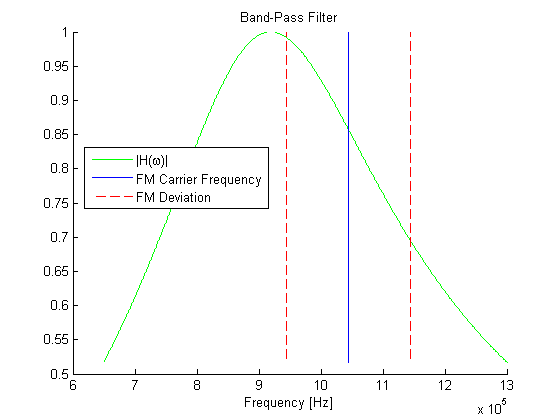
\includegraphics[width = 400px]{demod_matlab.png}
        \caption{Band-Pass Filter response in the region of interest.}
        \label{bpfm}
    \end{figure}
    
    \noindent Recall that $\mathcal{F}\{\frac{d}{dt}y(t)\} = j\omega Y(\omega)$, therefore taking a derivative is equivalent to passing $y(t)$ through a filter with frequency response $H(\omega) = j\omega$. We achieve a similar effect by using a band-pass filter with center frequency just below the carrier frequency of the FM signal. Since the FM signal's spectrum is located in the transition band of the filter, we are effectively multiplying it by $\approx -j\omega$ (See Figure~\ref{bpfm}). Since the transition band of the filter is not actually linear, it won't be a perfect derivative, but it is monotonically decreasing for frequencies above the passband, so the effect is similar. Another way to think about this process is to simply observe that, with the band-pass filter off-center, higher frequencies and lower frequencies in the FM signal will have different levels of attenuation, and thus the filtered signal will be enveloped by the message signal. \\
    \\
    Our realization of this filter is simply a voltage divider with $Z_1$ being a resistor and $Z_2$ being an LC tank. We chose $L = 1 \text{ }\mu$H and $C = 30$ nF which results in a band-pass filter centered at $\omega_0 \approx 2\pi\cdot 920$ kHz. We initially using $R = \frac{Q}{\omega_0 C} = 27 \text{ }\Omega$, but we found that doubling the quality factor and thus halving the resistor gave us better results.

    \subsection{Envelope Detection}
    After converting FM to AM, we use an envelope detector to extract the message signal from the AM signal. Our realization of the envelope detector is simply a diode biased around its built in potential followed by an RC LPF. The cutoff frequency of this filter can be chosen as low as 20 kHz (the highest audible frequency) since our message signal is audio, but we choose a cutoff frequency of $\omega_0 \approx 2\pi\cdot 160$ kHz because it was convenient given the components available. Since this cutoff frequency is far below the carrier frequency, it satisfies our needs.

    \subsection{Amplification}
    After extracting the message signal from the AM signal, we use a two-stage BJT amplifier to condition the signal in such a way that it can be played by an 8 $\Omega$ speaker.\\
    \\
    The first stage, which provides the gain, is a common emitter with resistive degeneration for stable DC biasing and capacitive degeneration for increasing high-frequency gain. We designed this amplifier by first choosing a bias current of $I_C = 1$ mA (which in turn sets $g_m = \frac{I_C}{v_t}$, where $v_t \approx 26$ mV is the thermal voltage constant), then setting $A_{DC} = 2$ and $A_{v} = 10$ and solving for $R_C = 260 \Omega$ and $R_E = 104 \Omega$. We chose $C_E = 100 \mu$F to be very large in order to increase the gain at all frequencies except DC. Biasing resistors were chosen to ensure the BJT remains in forward active mode and to keep the bias current at roughly 1 mA. \\
    \\
    The second stage, which buffers the signal, is an emitter follower.  Again, we first chose a bias current of $I_C = 1$ mA, which helped us solve for $R_E = 2.02$ k$\Omega$ and the biasing resistors. \\
    \\
    The filters at the input and output of the amplification block were chosen to pass audio frequencies. This constrains the operating band of the amplifier to (roughly) the interval [700 Hz, 160 kHz] (the lower bound is due to the HPF at the input and the upper bound is due to the LPF in the envelope detector).

\section{Results \& Discussion}

    \subsection{FM Demodulator}
    Upon construction of our FM Demodulator, we were successfully able to listen to FM signals generated in the lab. While it was difficult finding components with the exact values we calculated, we were able to modify our design and it still worked.
    
    \subsection{Transmission Lines}
    
    \begin{figure}[H]
        \centering
            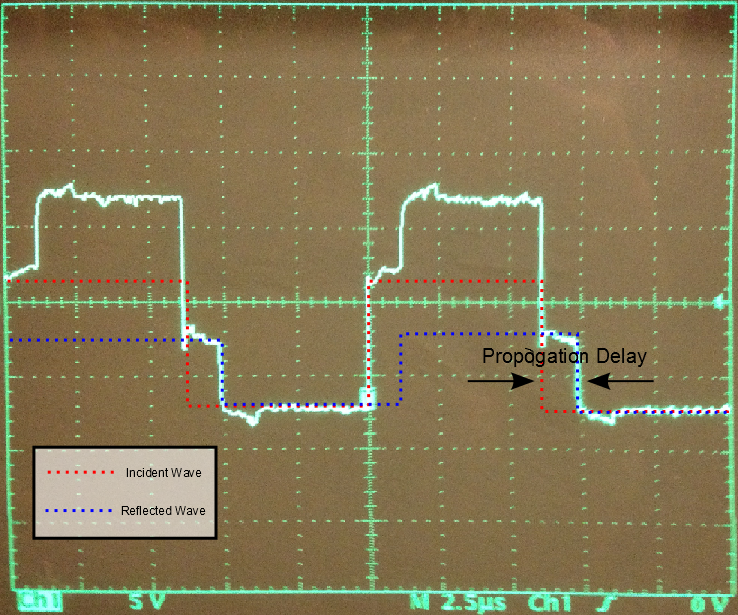
\includegraphics[width = 300px]{reflection.png}
        \caption{Reflection seen due to impedance mismatch on a transmission line.}
        \label{tline}
    \end{figure}
    
    We also investigated the properties of transmission lines. Specifically, we sent a square wave down a length of cable and estimated the length of cable given the propagation delay seen in the reflection (See Figure~\ref{tline}). We saw a 1.2 $\mu$s delay in sending the square wave and receiving the reflection, so the time it took the pulse to travel down the cable was roughly 0.6 $\mu$s, and if we estimate that the pulse travels at two-thirds of the speed of light, we can calculate the cable length $l$ as
    \begin{flalign*}
        l &= \frac{2}{3}\cdot c \cdot 0.6\cdot10^{-6} \\
        &= 120 \text{ meters.}
    \end{flalign*}
    We also estimated the characteristic impedance $Z_0$ of the cable to be $\approx 56 \Omega$ by terminating it with various resistors until there were no reflections.

    \subsection{Noise}
    For a demonstration of the Central Limit Theorem, please visit \\ \texttt{https://github.com/nosaesa/ugradio/tree/master/lab1/python}.

\section{Conclusion}
This lab proved to be very challenging and very rewarding. Radio is a fascinating topic and it was quite satisfying to design and build an FM receiver from the ground up. However, we do realize the shortcomings of such a simple design, and we look forward to revisiting the issue of receiving RF signals with more advanced equipment in the next lab.

\section{Acknowledgements}
We would like to thank: Ma\"{i}ssa Salama and Kevin Yu for their help in carrying out the work described above; Baylee Bordwell and Garret ``Karto'' Keating for their assistance; and Aaron Parsons for providing the opportunity and facilities necessary to perform these experiments.

\end{document}
